\chapter{Опис додатку з використанням кросс-платформених рішень}
\label{ch2}

\section{Структура проекту в React Native}
\label{section.2.1}

\begin{lstlisting}[style=light, language=Python,label={lst:rn_app_structure},caption=React Native App Layout]
├── App.js (1)
├── Readme.md
├── __tests__ (2)
│ └── App.js
├── android (3)
│ ├── app
│ ├── build
│ ├── build.gradle
│ ├── gradle
│ ├── gradle.properties
│ ├── gradlew
│ ├── gradlew.bat
│ ├── local.properties
│ └── settings.gradle
├── app.json (5)
├── babel.config.js (6)
├── index.js (7)
├── ios (4)
│ ├── BreedRN
│ ├── BreedRN.xcodeproj
│ ├── BreedRN.xcworkspace
│ ├── Podfile
│ ├── Podfile.lock
│ └── Pods
├── metro.config.js (8)
├── node_modules (11)
├── package-lock.json (10)
└── package.json (9)
\end{lstlisting}

\begin{enumerate}
    \item \textbf{App.js} сирцевий код нашого додатку
    \item \textbf{\_\_tests\_\_} сирцевий код тестів
    \item \textbf{android} сирцевий код платформеного коду Android
    \item \textbf{ios} сирцевий код платформеного коду iOS
    \item \textbf{app.json} конфігурує багато речей, від назви вашого додатка до піктограми до заставки, і навіть схеми глибоких зв’язків та ключів API для використання для деяких служб
    \item \textbf{babel.config.js} конфігурує Babel - це набір інструментів, який в основному використовується для перетворення коду ECMAScript 2015+ у зворотну сумісну версію JavaScript у поточних та старих браузерах або середовищах.
    \item \textbf{index.js} точка входу для React Native з цього файлу Javascript Engine вивантажує в пам'ять логіку додатку
    \item \textbf{metro.config.js} конфігурує Metro пакувальник JavaScript для платформ Android та iOS
    \item \textbf{package.json} конфігурує дерево залежностей або бібліотек, що використовує проект
    \item \textbf{package-lock.json} файл що описує повністю дерево залежностей, таким чином створює відтворюване середовище
    \item \textbf{node\_modules} репозиторій артефактів або сирцевого коду всіх Javascript пакетів, що використовує проект
\end{enumerate}

\section{Архітектура додатку React Native}
\label{section.2.2}
В реалізації додатку React Native ми використали систему звротніх викликів або так званих "хуків".
Наприклад, \textbf{useState} - це Хук, що дозволяє додавати стан React до функціональних компонентів.

"useState" оголошує "змінну стану" та повертає пару значень: поточний стан та функцію, яка його оновлює.
Наша змінна називається, data ми можемо називати її як завгодно, наприклад banana \ref{lst:rn_state_hooks}.

Використовуючи useEffect хук, ми повідомляємо React, що наш компонент повинен виконати додаткову фунцію після рендерингу.
React запам'ятає передану нами функцію (яку ми будемо називати "ефектом") і викличе її пізніше після оновлення UI нашого додатку.

Ефект котрий ми створили буде виконаний при ініціалізації додатку. І як результат виконання ми отримаємо дані з локальної бази які ми і відобразимо (див. на \ref{fig:rn_realm})).

\begin{figure}
    \begin{center}
        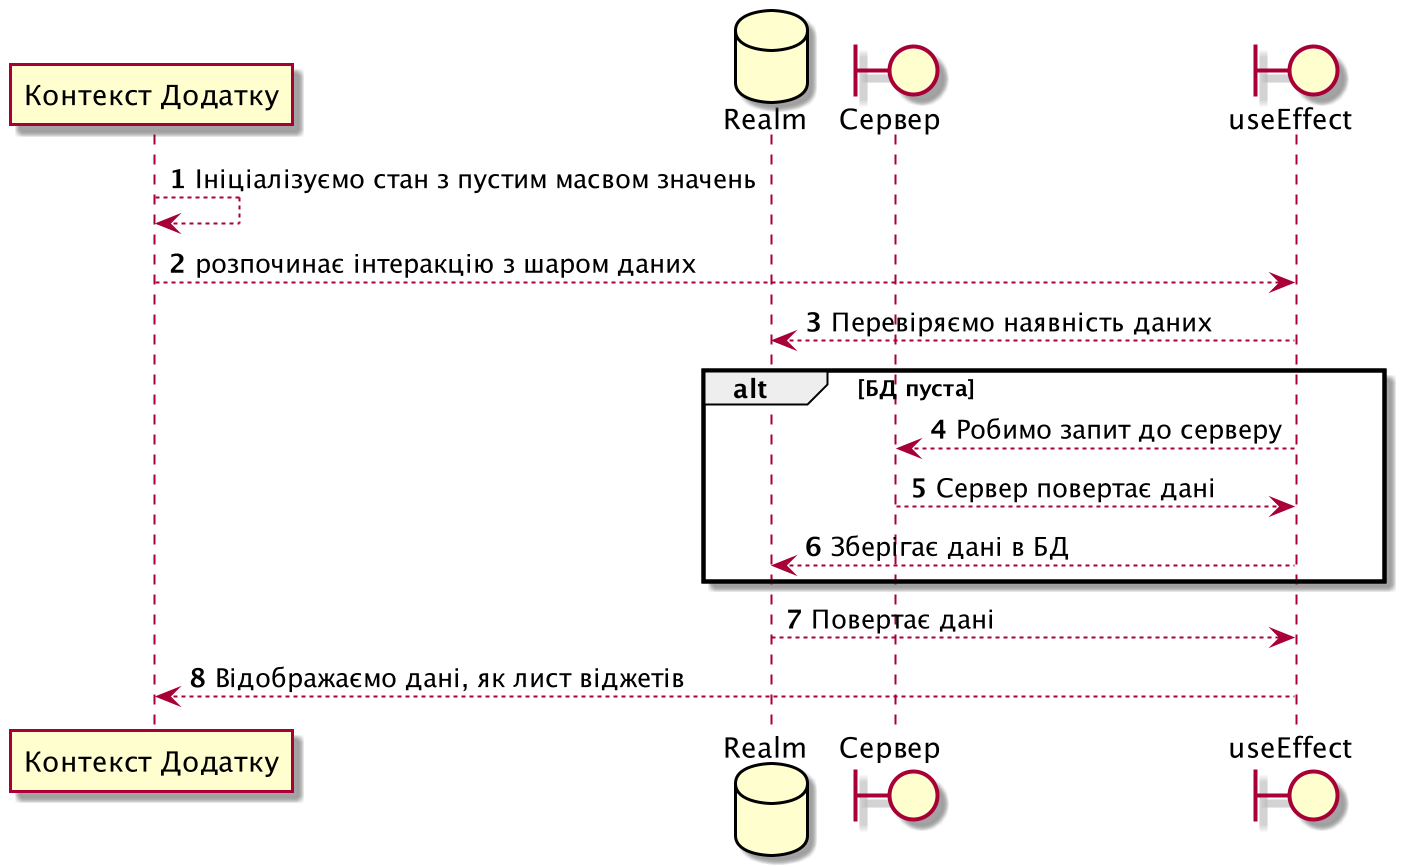
\includegraphics[scale=0.3]{app_widget.png}
        \caption{Схема послідовності віджету App та інтеракція з шаром даних}
        \label{fig:rn_realm}
    \end{center}
\end{figure}

\section{Використання Flutter http.dart в додатку}
\label{section.2.3}
В нашому додатку запит до інтернету описан в наступному описі сирцевого коду \ref{lst:flutter_networking}.

\begin{lstlisting}[style=light, language=Python,label={lst:flutter_networking},caption=Flutter Networking]
import 'dart:convert';

import 'package:breed_flutter/domain/breed.dart';
import 'package:http/http.dart' as http;
import 'package:http/http.dart';

class BreedApi {
  // 1
  Future<List<Breed>> fetchBreeds() async {
    // 2
    final Uri url = Uri.parse('https://dog.ceo/api/breeds/list/all');
    // 3
    final Response response = await http.get(url);
    // 4
    final Map<String, dynamic> body = jsonDecode(response.body);
    // 5
    final Map<String, dynamic> message = body['message'];

    // 6
    if (response.statusCode == 200) {
      // 7
      return message.keys.map((breedName) {
        final List<dynamic> rawRaces = message[breedName];
        final List<String> races =
            rawRaces.map((race) => race.toString()).toList();
        return Breed.make(name: breedName, races: races);
      }).toList();
    } else {
      // 8
      throw Exception('Failed to load breed items');
    }
  }
}
\end{lstlisting}

\begin{enumerate}
    \item Запит виконується асинхронно.
    \item Створюємо універсальний ідентифікатор ресурсу до REST API, що поверне список пород собак.
    \item Очікуємо результат виконання запиту до інтернету.
    \item Декодуємо JSON результат, як асоціативний масив з динамічними типом(тобто не визначений).
    \item Отримаємо значення по ключу "message".
    \item Перевіряємо статус. 200 значить успіх.
    \item Адаптуємо результат в конкретний підтип визначений, як головний контракт додатку.
    \item Якщо невдалий запит повертаємо помилку виконання.
\end{enumerate}

Найголовнішим принципом, котрим ми опируємо в прикладі запиту до інтернету, це використання "обіцянок" на базі dart:async Future<T>.
Асинхронні операції дозволяють нашій програмі завершити роботу, чекаючи закінчення іншої операції.
Результат використання Future API або закінчиться в завершенному стані або незавершенному.

Коли ми вперше виконуємо асинхрону функцію, то отримаємо посилання на незавершену дію, з якої ми очікуємо результат або помилку.
Щоб уникнути розповсюдження помилки до верхнів шарів ми маємо використати try/catch синтаксис.

Як видно з нашого прикладу використання пакету http.dart в по'єднанні з dart:async дає зручне та швидке розв'язання проблеми створення та прослухання результатів з інтернету.


\section{Запити до SQLite бази даних з sqflite}
\label{section.2.4}
Для рішення проблеми доступу до локальної бази даних на основі SQLite,
було використане одне з популярних рішень під назвою sqflite, яке підтримує iOS, Android та MacOS.

До можливостей sqflite можна віднести:

\begin{itemize}
    \item Підтримка транзакцій та пакетів.
    \item Помічники для вставки / запиту / оновлення / видалення запитів.
    \item Операції до БД, виконуються у фоновому потоці на iOS та Android.
    \item Підтримка Linux / Windows / DartVM за допомогою sqflite_common_ffi.
\end{itemize}

\begin{lstlisting}[style=light, language=Python,label={lst:flutter_sqflite},caption=Flutter SQFLITE]
import 'package:breed_flutter/domain/breed.dart';
import 'package:path/path.dart';
// 1
import 'package:sqflite/sqflite.dart';

class BreedDatabase {
  final Database database;

  BreedDatabase(this.database);

  static Future<BreedDatabase> create() async {
    // 2
    final Database database = await openDatabase(
      join(await getDatabasesPath(), 'doggie_database.db'),
      onCreate: (db, version) {
        // 3
        return db.execute(
          "CREATE TABLE breeds(id TEXT PRIMARY KEY, name TEXT, races TEXT, isFavorite INTEGER)",
        );
      },
      version: 1,
    );
    return BreedDatabase(database);
  }

  // 4
  Future<void> insert(Breed breed) async {
    await database.insert(
      'breeds',
      breed.toMap(),
      conflictAlgorithm: ConflictAlgorithm.replace,
    );
  }

  // 5
  Future<List<Breed>> all() async {
    final List<Map<String, dynamic>> maps =
        await database.query('breeds', orderBy: 'name');

    var list = List.generate(maps.length, (i) {
      return Breed.fromMap(maps[i]);
    });
    return list;
  }

  // 6
  Future<void> clear() async {
    await database.delete('breeds');
  }
}
\end{lstlisting}

\begin{enumerate}
    \item Імпортуємо пакет sqflite, котрий надає можливість створення об'єкту бази даних.
    \item Відкриваємо підключення до бази даних з використанням async/await API описаного в сексції \ref{section.3.3}
    \item SQL запит, що створіє таблицю під час створення SQL БД на файловій системі.
    \item Функція insert, що створює новий запис в таблиці використовуючи REPLACE стратегію для розв'язання конфліктів.
    \item Функція all, що повертає об'єкти з БД та перетворює на тип доменої логіки.
    \item Функція clear, знищує таблицю.
\end{enumerate}


\section{Управління станом з використанням Providers API}
\label{section.2.5}
Flutter пропонує кількп способів для управління станом. Серед них BLoC, Provider, Statefull Widgets, InheritedWidgets.
В даній роботі ми розглянемо Provider API, котрий взяв за основу систему InheritedWidgets(віджет, що наслідує).
Для того щоби зрозуміти контроль стану з Provider API ми повинні розлянути:

\begin{itemize}
    \item ChangeNotifier - це простий клас, включений до Flutter SDK, який забезпечує повідомлення про зміни своїх слухачів. Іншими словами, якщо щось є ChangeNotifier, ви можете підписатися на його зміни.
    \item ChangeNotifierProvider - це віджет, який надає екземпляр ChangeNotifier своїм нащадкам. Це походить від пакету провайдера.
    \item Consumer - це віджет, що дозволяє нам огорнути будь-який інший віджит далі в ієрархії та зчитати стан з класу, що наслідує ChangeNotifier.
\end{itemize}

В нашому додатку ми використали StateNotifier, котрий обновлює всіх підписників стану.
Так наприклад зміна значення з стану "завантажується" на стан "завантажений" приводить до перебудови віджету.

\begin{lstlisting}[style=light, language=Python,label={lst:flutter_sqflite},caption=Flutter SQFLITE]

// 1
class BreedListViewModel extends StateNotifier<BreedListState> {
  BreedListViewModel({required this.database})
      : super(const BreedListState.loading());
  final BreedDatabase database;

  Future<void> loadBreedList() async {
      // 2
      final List<Breed> cachedBreeds = await database.all();
      // 3
      state = BreedListState.loaded(savedBreeds);
  }
}

class BreedList extends StatefulWidget {
  BreedList({Key? key, required this.viewModel}) : super(key: key);
  final BreedListViewModel viewModel;

  @override
  _BreedListState createState() => _BreedListState();
}

class _BreedListState extends State<BreedList> {
  @override
  void initState() {
    super.initState();
    // 4
    widget.viewModel.loadBreedList();
  }

  @override
  Widget build(BuildContext context) {
    // 5
    return context
        .watch<BreedListState>()
        .when(loaded: showList, error: showError, loading: showLoading);
  }
}
\end{lstlisting}

\begin{enumerate}
    \item BreedListViewModel наслідує StateNotifier<BreedListState> отже стан описан додатковим дата класом BreedListState.
    \item Викликаючи loadBreedList() ми вигружаємо інформацію з БД.
    \item Встановлюємо новий стан, котрий буде поширен на віджет.
    \item Виконуємо виклик до моделі для, того щоб почати процес завантаження.
    \item Використовуючи API "watch" за рахунок StateNotifierProvider ми отримуємо новий стан, котрий оновлюємо згідно з трьох визначених типів.
\end{enumerate}


\section{Юніт тестування в Flutter}
\label{section.2.6}
Як було вже зазначено, найкращий спосіб контролю якості в проекті це написання та сопроводження коду написанням юнит тестів.
Цей підхід до розробки програмного забезпечення не оминув і розробку під Flutter.

В даній секції ми наведемо приклад тесту написаного для коду бізнес логіки.
Ми застосуємо пакети test та mockito.
Пакет тест надає доступ до функцій, які дозволяють нам групувати тести.
Пакет mockito надає функціонал, що дозволяє конфігурувати поведінку об'єктів типу mock(заглушка).
\begin{lstlisting}[style=light, language=Python,label={lst:flutter_unit_test},caption=Flutter Unit Test]
@GenerateMocks([BreedDatabase, BreedApi])
void main() {
  // 1
  final mockBreedDatabase = MockBreedDatabase();
  final mockBreedApi = MockBreedApi();

  // 2
  final listViewModel =
      BreedListViewModel(database: mockBreedDatabase, api: mockBreedApi);

  // 3
  final fakeDbBreed = Breed.make(name: "fakeDB");
  final fakeNetworkBreed = Breed.make(name: "fakeNetwork");

  // 4
  group('when toggle breed item', () {
    // 5
    setUp(() {
      when(mockBreedDatabase.all())
          .thenAnswer((_) => Future.value(<Breed>[fakeDbBreed]));
    });

    // 6
    test('should toggle breed and load new list items', () async {
      await listViewModel.toggleFavorite(fakeDbBreed);

      // 7
      var captured =
          verify(mockBreedDatabase.insert(captureAny)).captured.single;
      var capturedBreed = captured as Breed;

      // 8
      expect(capturedBreed.isFavorite, !fakeDbBreed.isFavorite);
    });
  });
\end{lstlisting}

\begin{enumerate}
    \item Створюємо об'єкти заглушки, що підміняють нам фактичний доступ до БД та API.
    \item Створюємо екземпляр моделі, що робить запит до інтернету та запусує/читає значення з БД.
    \item Створюємо екземпляри об'єктів, що репрезентують результат або з інернету, або з БД.
    \item Приклад застосування функції group з пакету test.
    \item Логіка, що виконується перед запуском тестів. Тут ми конфігуруємо поведінку моку.
    \item Безпосередньо сам тест з описом його приназначення.
    \item Ми перехоплюємо посилання на об'єкт, що ми плануємо зберігти в БД.
    \item Остання перевірка на то, що стан перехопленого об'єкту змінився.
\end{enumerate}

\section{Структура проекту в Flutter}
\label{section.2.7}

\begin{lstlisting}[style=light, language=Python,label={lst:flutter_project_layout},caption=Flutter Project Layout]
├── README.md
├── android (1)
│ ├── app
│ ├── build.gradle
│ ├── gradle
│ ├── gradle.properties
│ ├── gradlew
│ ├── gradlew.bat
│ ├── local.properties
│ └── settings.gradle
├── build (2)
├── ios (3)
│ ├── Flutter
│ ├── Podfile
│ ├── Runner
│ ├── Runner.xcodeproj
│ └── Runner.xcworkspace
├── lib (4)
│ ├── breed_list.dart
│ ├── data
│ ├── domain
│ ├── home.dart
│ ├── main.dart
│ └── presentation
├── pubspec.lock (5)
├── pubspec.yaml (6)
├── test (7)
│ ├── breed_database_test.dart
│ ├── breed_list_view_model_test.dart
│ ├── breed_list_view_model_test.mocks.dart
│ └── network_test.dart
└── web (8)
    ├── favicon.png
    ├── icons
    ├── index.html
    └── manifest.json
\end{lstlisting}

\begin{enumerate}
    \item \textbf{android} сирцевий код платформеного коду Android.
    \item \textbf{build} папка з тимчасовими файлами згенерованими Flutter CLI під час побудування проекту.
    \item \textbf{ios} сирцевий код платформеного коду iOS.
    \item \textbf{lib} сирцевий код Flutter, котрий фактично є серцем репозиторія та описую логіку проекту.
    \item \textbf{pubspec.lock} файл що описує повністю дерево залежностей, таким чином створює відтворюване середовище.
    \item \textbf{pubspec.yaml} конфігурує дерево залежностей або бібліотек, що використовує проект.
    \item \textbf{test} сирцевий код тестів для платформи Flutter.
    \item \textbf{web} сирцевий код платформеного коду веб сторінки.
\end{enumerate}
